\chapter{Neural Network Configuration}
\label{chapter:hyper}
\section{Hyperparameter Optimisation}

% \begin{table}[h!]
%     \centering
%     \begin{tabular}{|l|l|l|}
%     \hline
%     \textbf{Parameter} & \textbf{Type} & \textbf{Possible Values} \\ \hline
%     class\_weight & Boolean & True, False \\ \hline
%     training\_years & Choice & 2017\_2018\_2019, 2017 \\ \hline
%     kernel\_regularizer & Choice & l1l2, l1, l2 \\ \hline
%     spatial\_dropout & Choice & 0.3, 0.1, 0.5 \\ \hline
%     activation\_function & Choice & leaky\_relu, relu \\ \hline
%     pool\_size & Choice & 4, 2 \\ \hline
%     dropout & Choice & 0.3, 0.1, 0.5 \\ \hline
%     bias\_initializer & Boolean & True, False \\ \hline
%     learning\_rate & Choice & 0.001, 0.0001, 0.01 \\ \hline
%     loss\_function & Choice & binary\_focal\_crossentropy, binary\_crossentropy \\ \hline
%     \end{tabular}
%     \caption{Summary of initial hyperparameter search space.}
%     \label{tab:fixed_layers}
% \end{table}

\begin{table}
\caption{Summary of initial hyperparameter search space.}
\label{tab:fixed_layers}
\begin{tabular}{ll}
\toprule
name & values \\
\midrule
class\_weight & [true, false] \\
training\_years & ['2017\_2018\_2019', '2017'] \\
kernel\_regularizer & ['l1l2', 'l1', 'l2'] \\
spatial\_dropout & [0.3, 0.1, 0.5] \\
activation & ['leaky\_relu', 'relu'] \\
pool\_size & [4, 2] \\
dropout & [0.3, 0.1, 0.5] \\
bias\_initializer & [true, false] \\
learning\_rate & [0.001, 0.0001, 0.01] \\
loss\_function & ['binary\_focal\_crossentropy', 'binary\_crossentropy'] \\
\bottomrule
\end{tabular}
\end{table}



Table\,\ref{tab:fixed_layers} provides a summary of the search space for the initial hyperparameter tuning process. These parameters are critical as they influence the model's learning process, generalisation ability, and susceptibility to issues such as overfitting or bias. The chosen values in the search space represent a balance between exploring a wide range of options and focusing on promising areas based on prior knowledge or domain-specific considerations.

\begin{figure}[ht]
    \centering
    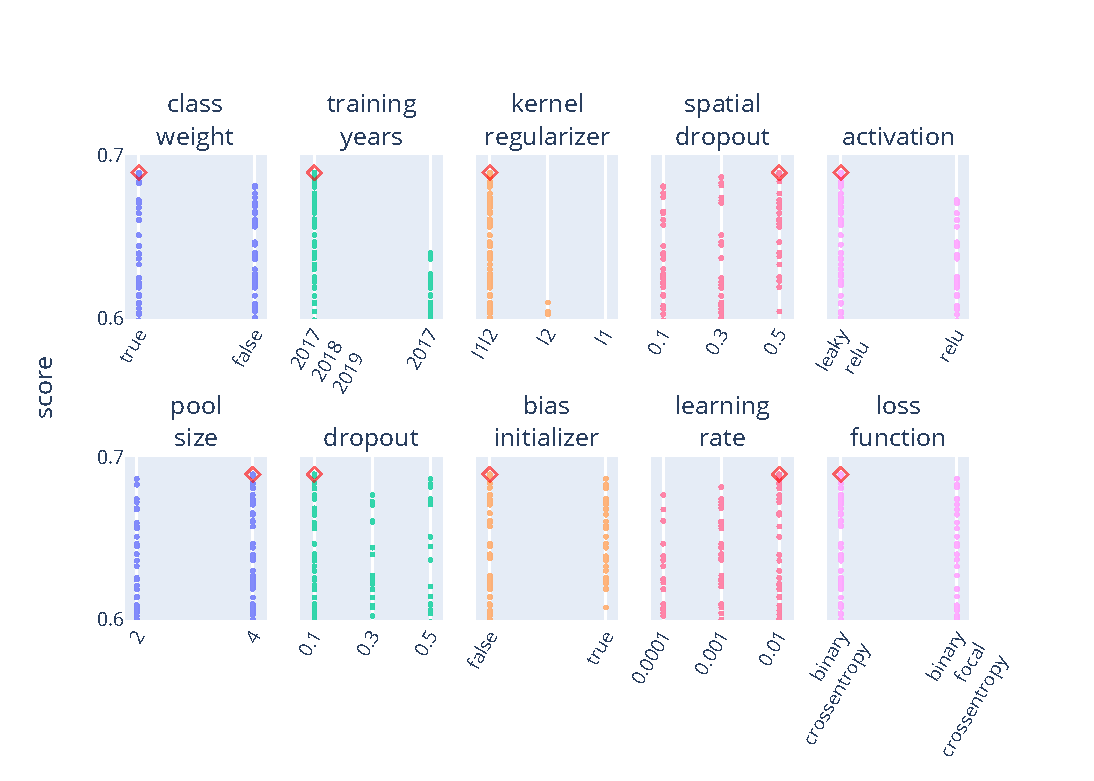
\includegraphics[width=0.9\linewidth, trim={10pt 10pt 40pt 40pt}, clip]{figures/figures_tuner/fixed_layers.pdf}
    \caption{The top f2-scores for the initial hyperparameter tuning process are highlighted, with the best score marked by a diamond shape.}
    \label{fig:fixed_layers}
\end{figure}

In the most successful trial, the model utilised training data from the medians of 2017, 2018, and 2019, applied L1L2 kernel regularization, used a spatial dropout rate of 0.5, and employed Leaky ReLU activation. The pool size was set to 4, dropout to 0.1, and bias initialization was disabled. The learning rate was 0.01, and the loss function was binary crossentropy, resulting in a score of 0.69.

While some of the initial trial's hyperparameters do not show significant overall improvement, some parameters do stand out. This is illustrated in Fig\,\ref{tab:fixed_layers}, particularly regarding training years, kernel regularization, activation function, and learning rate.